\documentclass[a4paper, 11pt, final, garamond]{book}
\usepackage{cours-preambule}
\usepackage{pdfpages}

\raggedbottom

\makeatletter
\renewcommand{\@chapapp}{Travaux pratiques -- TP}
\makeatother

\let\SavedIndent\indent
\protected\def\indent{%
  \begingroup
    \parindent=\the\parindent
    \SavedIndent
  \endgroup
}
\setlength{\parindent}{0pt}

\begin{document}
\setcounter{chapter}{14}

\chapter{Analyses spectrales de signaux \'electriques}

\section{Objectifs}

\begin{itemize} 
    \item Mettre en œuvre un dispositif expérimental illustrant l'utilité des
        fonctions de transfert pour  un système linéaire à un ou plusieurs
        étages.
    \item Étudier le filtrage linéaire d'un signal non  sinusoïdal à partir
        d'une analyse spectrale.
    \item Choisir un modèle de filtre en fonction d'un cahier des charges. 
\end{itemize}
 	
\section{S'approprier~: analyse spectrale}

\subsection{Décomposition en série de Fourier}

Toute fonction périodique peut se décomposer en série de Fourier, c'est-à-dire
en une somme de fonctions sinusoïdales de pulsations différentes. Soit $y$ une
fonction périodique de période $T$ et de pulsation $\w = 2\pi/T$. La
décomposition en série de Fourier de $y$ est~:

\[
    y(t) = y_0 + \sum_{n=1}^{\infty} a_n \cos(n\wt + \f)
\]

Avec $a_n$ et $\f_n$ respectivement l'amplitude et la phase de l'harmonique de
rang $n$.

Un logiciel tel que LatisPro (que l'on va utiliser ici) permet de réaliser
numériquement la décomposition en série de Fourier (en réalité une transformée
de Fourier numérique) d'un signal et de fournir une représentation graphique
exploitable.

\begin{minipage}{0.48\linewidth}
    \begin{center}
        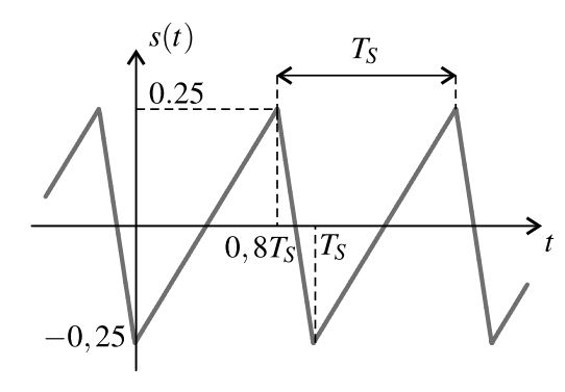
\includegraphics[height=5cm]{tp15_spectre-temp}
        \captionof{figure}{Représentation temporelle d'un signal périodique.}
    \end{center}
\end{minipage}
\hfill
\begin{minipage}{0.48\linewidth}
    \begin{center}
        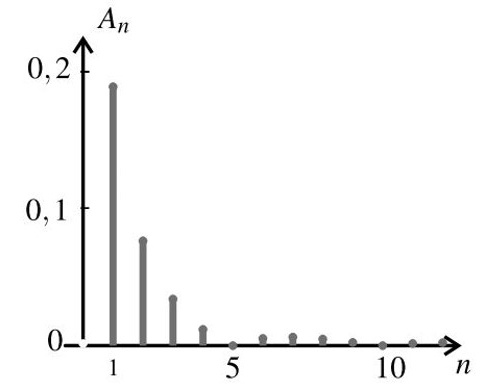
\includegraphics[height=5cm]{tp15_spectre-f}
        \captionof{figure}{Spectrogramme du même signal périodique.}
    \end{center}
\end{minipage}

\subsection{Vocabulaire}

\begin{itemize}
    \item Spectre~: représentation de l'amplitude de chacune des composantes
        spectrales d'un signal en fonction de leurs pulsations ou de leurs
        fréquences.
    \item $y_0 = \moy{y}$ est la valeur moyenne du signal $y$, c'est-à-dire sa
        \textbf{composante continue}~;
    \item $a_1 \cos(\wt + \f_1)$ est appelé
        \textbf{fondamental}~;
    \item $a_i \cos(n\wt + \f_i)$ est l'\textbf{harmonique} de
        rang $i$.
\end{itemize}

\begin{rrema}{Remarques}
    \begin{enumerate}
        \item Le fondamental est aussi l'harmonique de rang $1$.
        \item Le spectre d'un signal temporel pair ne contient que des
            harmoniques de rang pair ($n=2p, p\in\Nb$)
        \item Le spectre d'un signal temporel impair ne contient que des
            harmoniques de rang impair ($n=2p+1, p\in\Nb$)
    \end{enumerate}
\end{rrema}

\subsection{Durée d'enregistrement et fréquence d'échantillonnage}

Le critère de \textsc{Shannon} (vu en seconde année) impose que la
\textbf{fréquence d'échantillonnage} (fréquence de calcul) soit
\textbf{supérieure à deux fois la fréquence maximale du signal} étudié.
\bigbreak

Par ailleurs, le temps d'acquisition total $T_{\rm acq\, tot}$ doit être égal à
un multiple entier de fois la période du signal étudié~: $T_{\rm acq\, tot} =
nT$ avec $n\in \Zb$. Si ce n'est pas possible, il faut que la durée
d'acquisition soit longue, sachant que le pas fréquentiel du spectre vaudra~: 

\[
    \Delta f = \frac{1}{T_{\rm acq\, tot}}
\]

\section{Réaliser et valider}
\subsection{Analyses spectrales de signaux périodiques de différentes formes}
\subsubsection{Signal sinusoïdal}

\underline{Réaliser une acquisition}~: \bigbreak
\begin{enumerate}
    \item Connecter le générateur basses fréquences (GBF) à l'interface SYSAM
        entre les voies EA0 et la masse.
    \item Ouvrir le logiciel Latispro en suivant le chemin~: programmes
        $\rightarrow$ discipline $\rightarrow$ physique-chimie $\rightarrow$
        latispro.
    \item Allumer le GBF, choisir un signal sinusoïdal de fréquence
        $\SI{500}{Hz}$ et d'amplitude moyenne ($5-\SI{10}{V}$ par exemple).
    \item Pour faire une acquisition~: cliquer sur le bouton
        
\includegraphics[height=.5cm]{bouton_acq}
        \begin{itemize}
            \item \textit{Pour activer la voie EA0}~: Dans le cadre entrées
                analogiques, cliquer sur les boutons des entrées à activer (EA0
                ici~!).
            \item \textit{Pour paramétrer l'acquisition}~: Dans le cadre
                acquisition, onglet temporel, mode normal, entrer le nombre de
                points de mesure et la durée totale de l'acquisition. On
                choisira~:
                \begin{itemize}
                    \item Nombre de points~: $\num{10 000}$~;
                    \item Acquisition temporelle~; 
                \end{itemize}
                \begin{enumerate}[label=\sqenumi]
                    \item Durée totale d'acquisition $T_{\rm acq\, tot}$ à
                        choisir. Justifier ce choix succintement. 
                \end{enumerate}
                \begin{itemize}
                    \item Fin des réglages, vous êtes prêt-e à faire vos
                        enregistrements.
                \end{itemize}
            \item Lancer l'acquisition en cliquant sur
                
\includegraphics[height=.5cm]{bouton_lancer}
        \end{itemize}
\end{enumerate} \bigbreak

\underline{Tracer le spectre}~: \bigbreak
\begin{enumerate}
    \item Aller dans traitements $\rightarrow$ calculs spécifiques $\rightarrow$
        analyse de Fourier.
    \item Accéder à la liste des courbes gràce à
        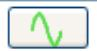
\includegraphics[height=.5cm]{bouton_courbe}
    \item Glisser la courbe et cliquer sur calcul.
\end{enumerate} \bigbreak
	
\underline{Commenter}~: \bigbreak
\begin{enumerate}[resume, label=\sqenumi]
    \item Quelle est l'allure du spectre~? Observez-vous des harmoniques~?
    \item En cliquant droit sur le graphe, prendre la loupe + pour zoomer,
        plusieurs fois si nécessaire ou utiliser le calibrage. Relever la
        fréquence fondamentale grâce à la fonction réticule (toujours en
        cliquant droit sur le graphe) et la comparer à celle indiquée par le
        GBF. Commenter l'éventuelle différence. 
\end{enumerate}

\subsubsection{Signaux triangulaires et carrés}

Changer la forme du signal délivré par le GBF en gardant la même fréquence
fondamentale et recommencer le même protocole. \bigbreak

\begin{enumerate}[resume, label=\sqenumi]
    \item Quelle est l'allure de chacun des spectres (signal triangulaire et
        carré)~? Observez-vous des harmoniques~?
    \item Quelle est la particularité de ces deux spectres~? Quelles sont leurs
        différences~?
\end{enumerate}

\subsection{Étude du spectre obtenu en sortie du filtre de Rauch}

On reprend le filtre de \textsc{Rauch} de la semaine précédente afin de filtrer
le signal carré. Notre objectif est d'obtenir à partir de ce signal un signal
sinusoïdal de \textbf{fréquence fondamentale double}. 

\begin{instruc}{Manipulation amplificateur}
    Connecter la borne \SI{+15}{V} du boitier à la sortie \SI{+15}{V} d'un
    générateur de tension continue, la borne \SI{-15}{V} du boitier à la sortie
    \SI{-15}{V} du générateur et le point milieu du boitier à la masse du
    générateur.
\end{instruc}

\begin{bror}{\includehand{-90}{0.8cm}}
    \centering\bfseries
    À la fin de la séance, on coupe le signal du GBF avant les alimentations de
    l'amplificateur opérationnel qui doivent être coupées en dernier.
\end{bror}

On réalise le montage en prenant $C=\SI{1}{nF}$ (cavalier prêt à être connecté
sur la boite) et $\alpha R$ est une boite de résistances variables. Le filtre a
été fabriqué avec $R= \SI{100}{k\Omega}$. \bigbreak

On s'intéresse tout d'abord au cas où $\alpha= 1$~: On prend donc $\alpha R =
\SI{100}{k\Omega}$. On injecte à l'entrée du filtre un signal créneau de
fréquence fondamentale $f_0$. \bigbreak

\begin{enumerate}[resume, label=\sqenumi]
    \item Comment choisir $f_0$ \textit{a priori} afin d'obtenir à partir de ce
        signal un signal sinusoïdal de \textbf{fréquence fondamentale double}~? 
\end{enumerate} \bigbreak

Choisir une durée d'enregistrement telle que $T_{\rm acq\, tot} = 2 T$, ou une
durée d'enregistrement très grande pour que l'analyse spectrale soit de bonne
qualité. Faire l'analyse spectrale du signal à l'entrée et à la sortie du
filtre. \bigbreak

\begin{enumerate}[resume, label=\sqenumi]
    \item Qu'observez-vous~? Quelle est l'allure du signal de sortie~?
\end{enumerate} \bigbreak

Refaire le même protocole pour $\alpha=\num{e-2}$~: on prend donc $\alpha R =
\SI{1000}{\Omega}$. On rappelle la fréquence de résonance trouvée la semaine
précédente dans ce cas est différente. \bigbreak

\begin{enumerate}[resume, label=\sqenumi]
    \item Quelle valeur faut-il alors choisir pour la fréquence fondamentale du
        créneau~? En déduire la valeur à donner à $T_{\rm acq tot}$.
\end{enumerate}

\section{Conclure}

\begin{enumerate}[resume, label=\sqenumi]
    \item Comparez les deux spectres de sortie. Interprétez les différences
        obtenues. Quel filtre permet d'atteindre l'objectif que l'on s'est
        initialement fixé~? 
\end{enumerate}

\end{document}
